\graphicspath{{./fig_PM/}}
%

\section{計算性能測定機能}
計算性能測定機能は,
ソルバー実行時に,プログラムコード内の測定対象部分の実行時間を測定し,
その統計情報を出力する機能を提供する.

各測定箇所は,整数値キー番号により識別される.
測定箇所はキー番号以外に,次のプロパティを持つ.
\begin{quote}
\begin{description}
\item[ラベル] 統計情報出力時のラベル文字列
\item[測定対象タイプ] 「計算時間」または「通信時間」
\item[排他測定フラグ] 「排他測定」または「非排他測定」
\end{description}
\end{quote}

\paragraph{測定対象タイプ}
測定を終了するstopメソッドには,オプションとして測定区間の「計算量」を
ユーザが自己申告できる機能がある.
測定対象タイプが計算時間の場合には,この申告量を浮動小数点演算量と解釈し,
統計情報出力時に計算速度(FLOPS値)を出力する.
一方,測定対象タイプが通信時間の場合には,申告量をバイト単位の通信量と解釈し,
統計情報出力時に通信速度(Byte/s単位)を出力する.

\paragraph{排他測定と非排他測定}
測定箇所は,排他測定フラグの真偽により,
「排他測定」と「非排他測定」とに分類される.
排他測定は,「(ほぼ)完成されたプログラムの実行時の状況を把握するために,
プログラムコードを排他的な領域に分割し,各領域の実行時間を測定する」
という使用方法を想定している.排他測定では,統計情報出力時に,
「全排他測定箇所の合計実行時間」に対する
「個々の排他測定箇所の実行時間」の割合も出力する.

一方,非排他測定は,プログラムのデバッグあるいはチューニング時に,一時的に
興味のある対象領域の実行時間を把握するのに使用することを想定している.
そのため,非排他測定区間は,排他測定区間や他の非排他測定区間と
重ねることも可能で,自由に設置できる.

\paragraph{並列実行時の制限}
並列実行時には,それぞれの排他測定区間は,並列計算ノードによらず同一回数だけ
実行されるものと仮定している.
計算ノード毎に実行回数が異なっていた場合には,
後述するprintメソッド実行時には,該当区間の統計情報は出力されない.

一方,非排他測定区間の設置には制限はなく,
並列計算ノード毎に実行回数が異なっていても問題ない.
非排他測定区間の測定結果の出力にはprintDetailメソッドを使用する.

%
\subsection{API説明}
計算性能測定機能は,
個々の測定箇所毎に時間測定を担当するPerfWatchクラスと,
全PerfWatchを管理して統計情報の計算と出力を担当するPerfMonitorクラス
により提供される.両クラスとも,Parallel\_Nodeクラスを継承している.
\begin{figure}[H]
\vspace{0.5cm}
\begin{center}
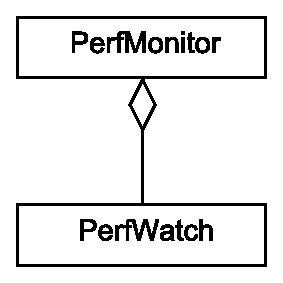
\includegraphics[width=0.15\textwidth]{PerfMonitor.eps}
\caption{計算性能測定機能 クラス図}
\label{fig:timing}
\end{center}
\end{figure}

PerfWatchクラスは,全てPerfMonitorクラスをとおして生成され操作されるので,
ソルバーから直接PerfWatchクラスのAPIを呼ぶことはない.

%
\subsubsection{PerfMonitorクラス公開メソッド}
\paragraph{初期化}\mbox{}\\
測定区間数({\tt nWatch})+1個の測定時計(PerfWatchクラス)をインスタンスして,
全計算時間用測定時計をスタートさせる.
測定区間を指定するキー番号は,0以上{\tt nWatch}未満である必要がある.
{\small
\begin{program}
void initialize(unsigned nWatch)
\end{program}
}

\paragraph{測定区間にプロパティを設定}\mbox{}\\
キー番号{\tt key}で識別される測定区間に,ラベル文字列{\tt label},
測定対象タイプ{\tt type}, 排他測定フラグ(true=排他測定/false=非排他測定)を設定.
{\small
\begin{program}
void setProperties(unsigned key, const string& label, Type type,
                   bool exclusive=true)
\end{program}
}

なお,測定対象タイプ{\tt type}の指定には,以下の定数を使用する.
\begin{quote}
\begin{description}
 \item[通信] {\tt PerfMonitor::COMM}   
 \item[計算] {\tt PerfMonitor::CALC}
\end{description}
\end{quote}

\paragraph{測定スタート}\mbox{}\\
キー番号{\tt key}で識別される測定区間の始まりを指定する.
{\small
\begin{program}
void start(unsigned key)
\end{program}
}

\paragraph{測定ストップ}\mbox{}\\
キー番号{\tt key}で識別される測定区間の終わりを指定する.
オプションとして,「タスク」あたりの計算量/通信量(バイト単位){\tt flopPerTask},
実行「タスク」数{\tt iterationCount}を申告できる.
{\small
\begin{program}
void stop(unsigned key, SKL_REAL flopPerTask=0.0, unsigned iterationCount=1)
\end{program}
}

\paragraph{測定結果の集約}\mbox{}\\
測定結果情報をノード0に集約し,統計情報を計算する.
また,初期化時にスタートさせた全計算時間用測定をストップさせる.
{\small
\begin{program}
void gather()
\end{program}
}

\paragraph{測定結果の出力}\mbox{}\\
排他測定区間についての統計情報を出力する.
ノード0以外では, 呼び出されてもなにもしない.
{\small
\begin{program}
void print(FILE* fp)
\end{program}
}

\paragraph{詳細な測定結果の出力}\mbox{}\\
非排他測定区間も含めて,詳細な統計情報を出力する.
ノード0以外では, 呼び出されてもなにもしない.
{\small
\begin{program}
void printDetail(FILE* fp)
\end{program}
}

%
\subsection{PerfMonitorクラスの使用方法}
PerfMonitorクラスを使用するには,ヘッダファイルPerfMonitor.hインクルードする.
また,並列化時にはMPI\_Init(), MPI\_Finalize()はユーザプログラムの管理で行うこと.

\paragraph{初期化}\mbox{}\\
以下の8ステップが必要:
\begin{enumerate}
\item インスタンス化
\item 測定番号識別キー番号定数の用意
\item initializeメソッドによる測定区間数の登録
\item setRankInfoメソッドによる並列ランク情報の設定
\item setPropertiesメソッドによる各測定区間へのプロパティの設定
\end{enumerate}

{\small
\begin{program}

  int my_rank; // 自ノードのランク番号
  …
  // (1) インスタンス化
  PerfMonitor PM
  …
  // (2) 測定番号識別キー番号定数
  enum timing_key {
    tm_sec1,
    tm_sec2,
    … 
    tm_secN,
    tm_END_,   // ターミネータ(=測定区間総数)
  };

  …
  // (3) 並列情報設定
  PM.setRankInfo(my_rank);

  // (4) 測定区間数の登録
  PM.initialize(tm_END_);

  // (5) 各測定区間にプロパティを設定
  PM.setProperties(tm_sec1, "SEC1", PerfMonitor::CALC);       //計算,排他
  PM.setProperties(tm_sec2, "SEC2", PerfMonitor::COMM);       //通信,排他
  PM.setProperties(tm_sec3, "SEC3", PerfMonitor::CALC, false);//計算,非排他
  …
\end{program}
}

\paragraph{測定区間の指定}\mbox{}
単純な指定では,
測定対象区間を同一キーを指定したstartメソッドとstopメソッドで挟む.
{\small
\begin{program}
  PM.start(tm_sec1);

  /* 測定対象区間 */

  PM.stop(tm_sec1);
\end{program}
}

以下の例では,測定対象区間内で
浮動小数計算量{\tt flop}のブロックを{\tt nStep}回実行していることを申告してる.
{\small
\begin{program}
  PM.start(tm_sec1);

  for (int i = 0; i < nStep; i++) {
    /* このブロックの浮動小数計算量が flop */
  }

  PM.stop(tm_sec1, flop, nStep);
\end{program}
}

\paragraph{測定結果の集計・出力}\mbox{}\\
測定結果出力メソッドを呼び出す前に,全ノードで集計メソッドgatherを呼び出す
必要がある.
出力メソッドはprintおよびprintDetailは,ノード0から呼ばれた時のみ
指定されたファイルへ測定結果情報を出力する.
{\small
\begin{program}
  // 測定結果の集計(gathreメソッドは全ノードで呼ぶこと)
  PM.gather();

  // コンソールへの測定結果の出力
  // (printとprintDetailメソッドはノード0以外は呼ばれても何もしない)
  PM.print(stdout);
  PM.printDetail(stdout);

  if (p.ID == 0) {
    FILE* fp = fopen("timing.txt", "w");

    // ファイルへの測定結果の出力
    // (printとprintDetailメソッドは, ノード0のみから呼び出してもOK)
    PM.print(fp);
    PM.printDetail(fp);

    fclose(fp);
  }
\end{program}
}

\paragraph{クラス変数TimingLevelによる測定レベル制御}\mbox{}\\
クラス変数TimingLevelの内容を
\[
\textrm{TimingLevel} = \left\{
\begin{array}{ll}
 0 & \textrm{測定なし}\\
 1 & \textrm{排他測定のみ実行}\\
 2 & \textrm{非排他測定も実行}
\end{array}
\right.
\]
と設定することにより,ヘッダファイルPerfMonitor.h内で定義された
2つのマクロPM\_TIMING\_\_,PM\_TIMING\_DETAIL\_\_をとおして,
ソルバー実行時の測定レベルを制御できる.
\begin{quote}
\begin{alltt}
#define PM_TIMING__         if (PerfMonitor::TimingLevel > 0)
#define PM_TIMING_DETAIL__  if (PerfMonitor::TimingLevel > 1)
\end{alltt}
\end{quote}

{\small
\begin{program}
   …
PM_TIMING__ { MO.start(...); }

   /* 排他測定区間 */

PM_TIMING__ { MO.stop(...); }
   …
   …
PM_TIMING_DETAIL_ { MO.start(...); }

   /*  非排他測定区間  */

PM_TIMING_DETAIL_ { MO.stop(...);
\end{program}
}

%
\subsection{統計情報出力内容}
\paragraph{printメソッド出力内容}\mbox{}\\
「{\tt Report of Timing Statistics}」に続いて

\begin{quote}
\begin{description}

\item[\tt Total execution time]\mbox{}\\
 ノード0における,initializeメソッド呼び出しからgatherメソッド呼び出しまでの時間
 
\item[\tt Parallel Mode]\mbox{}\\
 並列実行モードと,そのプロセス,スレッド数
 
\item[\tt Total time of measured sections]\mbox{}\\
 全排他測定区間における「積算実行時間のノード間平均」の合計
\end{description}
\end{quote}


「{\tt Statistics per MPI process [Node Average]}」に続いて,各排他測定区間毎に

\begin{quote}
\begin{description}
\item[\tt call]\mbox{}\\
 測定回数(「startメソッド〜stopメソッド」ペアの呼び出し回数)
\item[\tt accumulated time]\mbox{}\\
 積算実行時間({\tt avr[sec]}はノード間平均値,
{\tt avr[\%]}は「{\tt Total time of measured sections}」値に対する平均値の割合,
{\tt sdv[sec]}は標準偏差,
{\tt avr/call[sec]}は1測定あたりの平均値)
\item[{\tt flop | messages[Bytes]}]\mbox{}\\
積算浮動小数演算量または通信量({\tt avr}はノード間平均値,
{\tt speed}は積算実行時間のノード間平均値より求めた計算速度または通信速度)
\end{description}
\end{quote}

なお,排他測定区間における測定回数がノード毎に異なっていた場合には,
その排他測定区間に関する統計情報の計算は行われず,「{\tt NA}」と出力される.

以下に表示例を示す.

{\small
\begin{program}
Report of Timing Statistics

Parallel Mode                    :   Hybrid (2 processes x 4 threads)

Total execution time            = 4.212366e+00 [sec]
Total time of measured sections = 4.160442e+00 [sec]

Statistics per MPI process [Node Average]
Label                  | call |            accumulated time        |         flop | messages[Bytes]
                       |      |  avr[sec] avr[%] sdv[sec] avr/call |   avr      sdv         speed
-----------------------+------+------------------------------------+---------------------------------
Projection_Velocity    : 4231   2.120e+00  50.9 5.288e-03 5.01e-04  2.99e+10  0.00e+00   13.15 Gflops
Poisson_SOR2_SMA       : 8462   8.246e-01  19.8 2.962e-02 9.74e-05  9.98e+09  0.00e+00   11.27 Gflops
Pseudo_Velocity        :   50   4.601e-01  11.0 7.571e-03 9.20e-03  2.61e+09  0.00e+00    5.29 Gflops
Sync_Pressure          : 8462   2.605e-01   6.2 7.657e-03 3.07e-05  2.77e+08  0.00e+00 1015.04 MB/sec
Poisson_Norm_Div_max   : 4231   1.144e-01   2.7 1.891e-03 2.70e-05  1.38e+09  0.00e+00   11.28 Gflops
Projection_Velocity_BC : 4231   1.107e-01   2.6 1.099e-02 2.61e-05  1.56e+08  0.00e+00    1.31 Gflops
A_R_Poisson_Residual   : 8462   6.619e-02   1.5 2.739e-02 7.82e-06  1.35e+05  0.00e+00    1.95 MB/sec
assign_Const_to_Array  : 4281   5.136e-02   1.2 1.367e-03 1.19e-05  0.00e+00  0.00e+00    0.00 Mflops
A_R_Poisson_Norm       : 4231   4.450e-02   1.0 1.369e-02 1.05e-05  1.35e+05  0.00e+00    2.90 MB/sec
Copy_Array             :  100   1.937e-02   0.4 2.990e-04 1.93e-04  0.00e+00  0.00e+00    0.00 Mflops
Divergence_of_Pvec     :   50   1.908e-02   0.4 5.264e-05 3.81e-04  1.83e+08  0.00e+00    8.95 Gflops
Sync_Pseudo_Velocity   :   50   1.709e-02   0.4 7.433e-03 3.41e-04  9.83e+06  0.00e+00  548.29 MB/sec
Variation_Space        :   50   1.561e-02   0.3 3.702e-04 3.12e-04  8.19e+07  0.00e+00    4.89 Gflops
Search_Vmax            :   50   8.687e-03   0.2 2.927e-03 1.73e-04  2.94e+07  0.00e+00    3.16 Gflops
Pvec_Euler_Explicit    :   50   5.660e-03   0.1 1.177e-04 1.13e-04  2.62e+07  0.00e+00    4.31 Gflops
Sync_Velocity          :   50   5.069e-03   0.1 3.446e-05 1.01e-04  3.93e+07  0.00e+00    7.22 GB/sec
-----------------------+------+------------------------------------+----------------------------------
Total                  |        4.1604e+00                             4.441e+10           9.94 Gflops
   Performance         |                                                                  39.77 Gflops
\end{program}
}

\paragraph{printDetailメソッド出力内容}
各測定区間,各ノード毎に,以下を出力
\begin{quote}
\begin{description}
\item[{\tt accm[s]}]\mbox{}\\
積算実行時間
\item[{\tt accm[\%]}]\mbox{}\\
積算実行時間の「{\tt Total time of measured sections}」値に対する割合
\item[{\tt waiting[s]}]\mbox{}\\
待ち時間(「積算実行時間のノード間最大値」と「積算実行時間」の差)
\item[{\tt accm/call[s]}]\mbox{}\\
1測定あたりの実行時間
\item[{\tt flop|msg}]\mbox{}\\
積算浮動小数演算量または通信量(バイト単位)
\item[speed]\mbox{}\\
積算実行時間より求めた計算速度または通信速度
\end{description}
\end{quote}

なお,非排他測定区間については,ラベル文字列をその前に「{\tt *}」をつけて表示する.

以下に表示例を示す.

{\small
\begin{program}

Pseudo_Velocity
                call       accm[s] accm[%]    waiting[s]  accm/call[s]    flop|msg     speed
#0    :           50  4.513264e-01   10.85  1.812696e-02  9.026527e-03   2.615e+09     5.40 Gflops
#1    :           50  4.579675e-01   11.01  1.148582e-02  9.159350e-03   2.615e+09     5.32 Gflops
#2    :           50  4.694533e-01   11.28  0.000000e+00  9.389067e-03   2.615e+09     5.19 Gflops
#3    :           50  4.618225e-01   11.10  7.630825e-03  9.236450e-03   2.615e+09     5.27 Gflops

A_R_Vmax
                call       accm[s] accm[%]    waiting[s]  accm/call[s]    flop|msg     speed
#0    :           50  3.278255e-04    0.01  8.788824e-03  6.556511e-06   1.600e+03     4.65 MB/sec
#1    :           50  3.207922e-03    0.08  5.908728e-03  6.415844e-05   1.600e+03   487.08 KB/sec
#2    :           50  3.243446e-03    0.08  5.873203e-03  6.486893e-05   1.600e+03   481.74 KB/sec
#3    :           50  9.116650e-03    0.22  0.000000e+00  1.823330e-04   1.600e+03   171.39 KB/sec

\end{program}
}



